% Copyright (c) 2014,2016 Casper Ti. Vector

\chapter{系統軟體測試}

本論文將開發讓商家能夠結合商品與RFID標籤,以達到快速建構與管理商品資料庫之系統,並且讓商家及顧客可以運用手機NFC功能來實際運作比特幣的行動支付流程。店家只需要掃描商品上的RFID標籤,即可快速建立交易清單,再利用NFC功能與顧客之行動裝置進行訊息交換,輕鬆地將商家的收款地址以及交易資料傳送給顧客,收到資料後便能快速地以顧客之比特幣行動電子錢包付款,並將交易細項儲存下來,以便未來商家與顧客能夠快速查詢比特幣行動支付的交易紀錄。
本系統主要是以完成區塊鏈之數位加密貨幣的收款監督系統為主要目標,本論文進而將積極利用自由軟體的利基:使用成本低、進入門檻低、開放原始碼、社群能力強、共通性及移植性強、資通安全性高等優勢來開發本論文收款監督系統的應用服務平台。
本專案範圍包含建置下面主系統與各項子系統,主系統為:
		\paragraph{區塊鏈的實名交易監督系統(Blockchain Real-name Transaction Monitoring System, BRTMS)}

各子系統分別為:
 		\paragraph{商家端建置與管理商品資訊子系統(Store and Merchandise Information Management Sub-System,SMIMSS)}本系統可以讓商家在進貨時,快速地將RFID標籤之識別碼與進貨商品資訊整合在一起,並且透過本系統新增、修改或刪除資料庫內部的資訊,包括產品名稱、詳細資訊,存貨數量等資訊,商家與顧客便可依照該資料庫取得當前商品資訊與狀態。不僅讓商店的存貨資訊更加清楚明瞭,也可以提供顧客更多的即時服務。
 		\paragraph{商家端行動收銀與交易明細系統(Store Mobile payment Collection and Transaction Sub-System,SMCTSS)}本系統使商家在結帳時,能夠以手機NFC功能掃描商品上的RFID 標籤,即可簡單地建立交易清單,並透過NFC與顧客手機碰觸,將交易清單以及商家之比特幣收款地址等等重要交易資訊一併傳遞給顧客,可以簡短結帳的速度,使結帳效率大幅提升。 
 		\paragraph{顧客端行動支付與交易明細系統(Client Mobile Payment and Transaction Sub-System,CMPTSS)}顧客在結帳時,不必再麻煩的拿出信用卡或是零錢包,只需要拿出手機讓店員以NFC將交易清單與比特幣地址轉送給自己,即可自動連結至比特幣電子錢包的應用程式當中,並且自動填妥相關資料,如:交易金額、收款地址等等與此同時也能將交易紀錄儲存於客戶端,以便日後顧客快速取得過往的交易紀錄,除此之外亦可讓廣大的民眾體驗數位加密貨幣與行動支付帶來的便利生活。

 	\section{測試說明}

 		\subsection{測試範圍}本文件主要是描述區塊鏈的實名交易監督系統的測試計畫。確認在系統整合前,必須先確認所有的設計元件均可正確的輸出,在此我們著重於整合系統測試 (Integration Test) 及接受測試 (Acceptance Test)。本文件內容將依據系統需求規格書與系統設計文件,描述關於整合測試的相關計畫與內容。並希望透過此文件之描述與實踐,達到順利進行測試工作之目的。

 		\subsection{接受標準}本測試計劃需要滿足下列的測試接受準則: 

 			\begin{enumerate}
				\item 本系統需要對所有列為必要(Critical、Important、Desirable)之需求作完整測試。
				\item 測試程序需要依照本測試計畫所訂定的程序進行,所有測試結果需要能符合預期測試結果方能接受。
				\item 以測試案例為單位,當測試未通過時,需要進行該單元的測試,其接受的準則與前一項規定相同。 
			\end{enumerate}
 	
 	\section{測試環境}

 		\subsection{硬件規格}
 			
 			\paragraph{系統主機}一台以上主機,每台主機CPU為Intel P4 1.0GHz或以上,256 MB RAM或以上,60G以上硬碟空間。
 			\paragraph{周邊設備}一台以上智慧型手機,與用來代表虛擬商品的數個RFID標籤;已可供測試NFC用的智慧型手機包含小米3 WCDMA版,詳細規格於表\ref{mi},Google Nexus 5X,詳細規格於表\ref{5x}。
	 			\begin{table}[htbp]
				\centering
				\caption{小米3手機規格}
				\label{mi}
				\begin{tabular}{|l|l|}
				\hline
				系統頻率 & GSM四頻、WCDMA \\ \hline
				作業系統 & Android 4.3 \\ \hline
				處理器 & Qualcomm Snapdragon 800 2.3 GHz四核心 \\ \hline
				記憶體 & 2GB RAM、16GB ROM \\ \hline
				記憶卡 & 不支援 \\ \hline
				顯示螢幕 & 5吋1670萬色IPS(1920×1080 pixels)、441ppi \\ \hline
				相機 & 1300萬畫素(F2.2、28mm)、200萬副鏡頭、1080p \\ \hline
				電池 & 3050 mAh(不可換) \\ \hline
				尺寸 & 144x73.6x8.1mm \\ \hline
				重量 & 145g \\ \hline
				\end{tabular}
				\end{table}

				\begin{table}[htbp]
				\centering
				\caption{Google Nexus 5X手機規格}
				\label{5x}
				\begin{tabular}{|l|l|}
				\hline
				系統頻率 & GSM四頻、WCDMA \\ \hline
				作業系統 & Android 6.0 \\ \hline
				處理器 & Qualcomm Snapdragon 800 1.8 GHz 六核 \\ \hline
				記憶體 & 2GB RAM、16GB ROM \\ \hline
				記憶卡 & 不支援 \\ \hline
				顯示螢幕 & 5吋1670萬色IPS(1920×1080 pixels)、441ppi \\ \hline
				相機 & 1300萬畫素(F2.2、28mm)、200萬副鏡頭、1080p \\ \hline
				電池 & 2,700 mAh(不可換) \\ \hline
				尺寸 & 147x72.6x7.9mm \\ \hline
				重量 & 136g \\ \hline
				\end{tabular}
				\end{table}

 		\subsection{軟件規格}
 		關於測試環境所需的軟體規格說明,如下列所示:作業系統:Window 10、Android 6.0.1/7.1.1

 		\subsection{測試數據源}
 		在銘傳大學桃園校區資工系實驗室,由本計畫主持人及助理人員透過Android手機進行的交易模擬實驗,測試環境如圖\ref{fig4}的示意。

 	\section{測試計劃和程序}

 		\subsection{測試時間規劃}

 		\paragraph{時程}

 			\begin{enumerate}
 				\item 各子系統之內部元件整合測試 (Module Test)(106/2/25~106/6/8)
 				\item 區塊鏈的實名交易監督系統整合測試 (Integration Test) (106/6/8~106/6/21)
 				\item 區塊鏈的實名交易監督系統接受度測試 (Acceptance Test) (106/7/10~106/7/21)
			\end{enumerate}

		\paragraph{查核點}

			\begin{enumerate}
 				\item 各子系統之內部元件整合測試 (Module Test)(106/5/10)
 				\item 區塊鏈的實名交易監督系統整合測試 (Integration Test) (106/7/1)
 				\item 區塊鏈的實名交易監督系統接受度測試 (Acceptance Test) (106/7/1)
 			\end{enumerate}

 		\subsection{整合測試(Integration Testing)}
 			\begin{figure}[htbp]
				\centering
				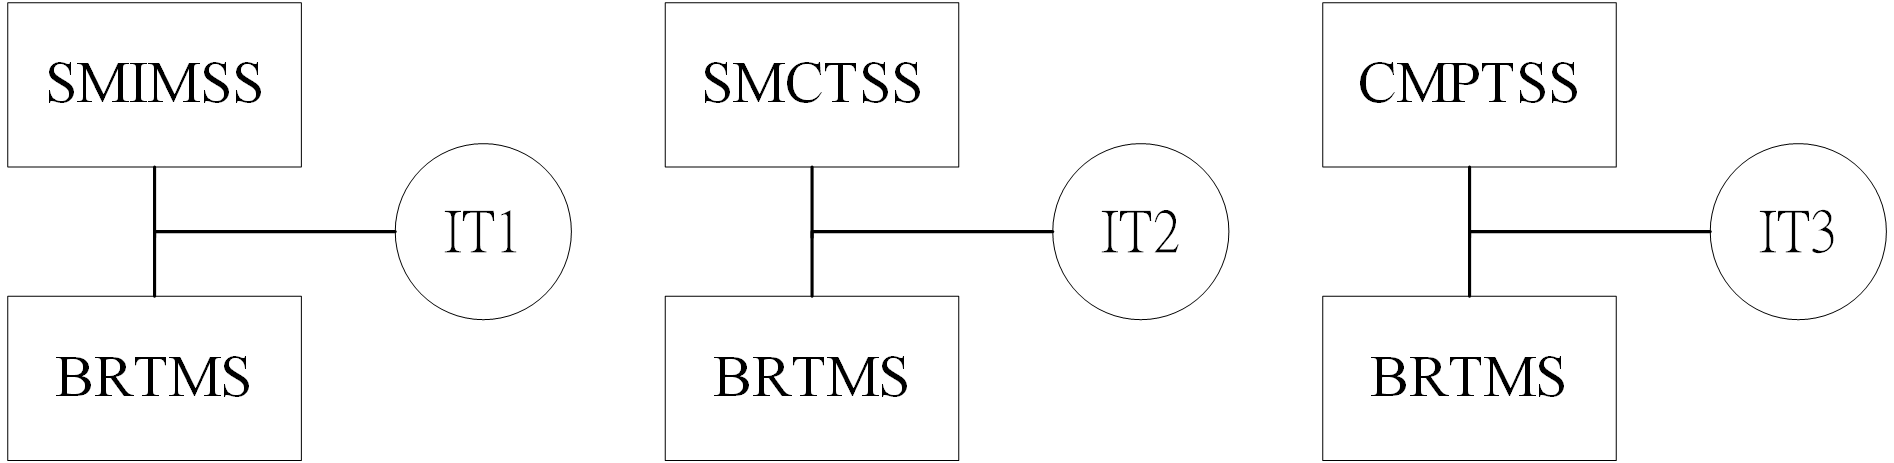
\includegraphics[width = 1\textwidth]{IntegrationTesting.png}
				\caption{整合子系統測試}\label{IntegrationTesting}
			\end{figure}

		\subsection{接受測試(Acceptance Testing,AT)}
		本系統須達成以下三組接受用況陳列的所有功能,測試本論文搭設計與搭建的系統功能是否能夠順利運行
		。測試的角色有兩個,分別為管理員以及使用者,如圖\ref{usecasediagram}為BRTMS用況示意圖,預計測試服務器的組態設定、手機的組態設定以及數據庫的組態設定:
			\begin{figure}[htbp]
				\centering
				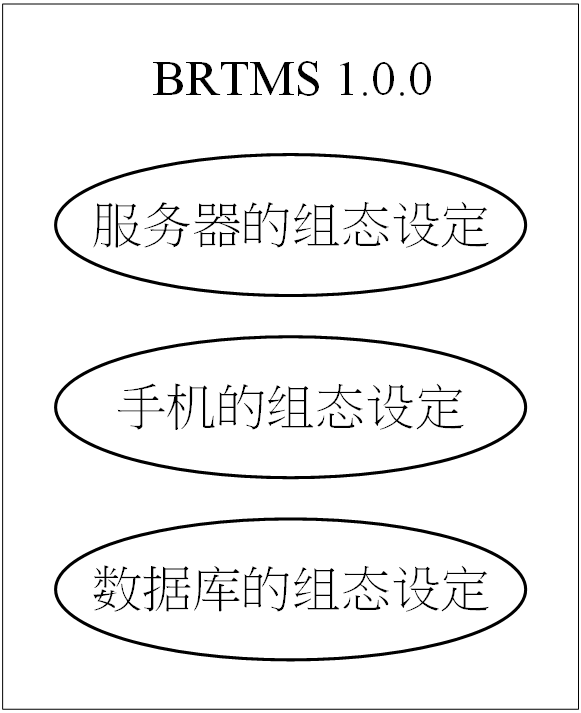
\includegraphics[width = 0.6\textwidth]{usecasediagram.png}
				\caption{BRTMS使用用況圖 (use case diagram)}\label{usecasediagram}
			\end{figure}
		圖\ref{AcceptanceTesting}為三組接受測試的示意圖,對本區塊鏈的實名交易監督系統進行測試。
			\begin{figure}[htbp]
				\centering
				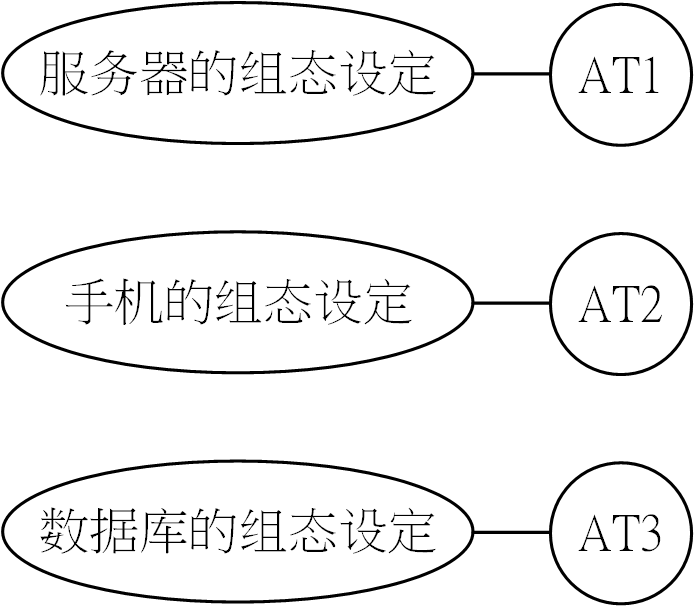
\includegraphics[width = 0.4\textwidth]{AcceptanceTesting.png}
				\caption{接受測試(Acceptance Testing)}\label{AcceptanceTesting}
			\end{figure}

		\section{测试用況(Test Case)}
			\subsection{集成测试(Integration Test)}
				
			\paragraph{IT1 测试用況}
				表\ref{IT1TestCase}為IT1 测试用況,測試對象為商家端建置與管理商品資訊子系統。目的:驗證〔SMIMSS 1.1.0〕子系統能否正確管理商品資訊。

				\begin{table}[htbp]
				\centering
				\caption{IT1 Test Case}
				\label{IT1TestCase}
				\begin{tabular}{|l|l|}
				\hline
				Identification & IT1 \\ \hline
				Name & 整合SMIMSS至BRTMS \\ \hline
				Tested target & {[}SMIMSS 1.1.0{]}、{[}BRTMS 1.0.0{]} \\ \hline
				Reference & SMIMSS-F-001$\sim$ SMIMSS-F-005 \\ \hline
				Severity & 1(Critical) \\ \hline
				\multirow{5}{*}{Instructions} & 1.     能夠新增店家帳戶 \\ \cline{2-2} 
				 & 2.     能夠新增/修改/刪除店員帳戶 \\ \cline{2-2} 
				 & 3.     能夠新增/刪除/修改商品資訊 \\ \cline{2-2} 
				 & 4.     能夠取得產品資訊 \\ \cline{2-2} 
				 & 5.     能夠接收交易資訊 \\ \hline
				\multirow{5}{*}{Expected result} & 1.     成功新增店家帳戶 \\ \cline{2-2} 
				 & 2.     成功新增/修改/刪除店員帳戶 \\ \cline{2-2} 
				 & 3.     成功新增/修改/刪除商品資訊 \\ \cline{2-2} 
				 & 4.     成功取得產品資訊 \\ \cline{2-2} 
				 & 5.     成功接收交易資訊 \\ \hline
				Cleanup & 無 \\ \hline
				\end{tabular}
				\end{table}


			\paragraph{IT2测试用況}
				表\ref{IT2TestCase}為IT2 测试用況麽目標,測試對象為商家端行動收銀與交易明細系統。目的:驗證〔SMCTSS 1.2.0〕子系統是否能夠完成一筆行動支付之交易。

					\begin{table}[htbp]
					\caption{IT2 Test Case} % title of Table
					\centering % used for centering table
					\label{IT2TestCase} % is used to refer this table in the text
					\begin{tabular}{|l|l|}
					\hline
					Identification & IT2 \\ \hline
					Name & 整合SMCTSS至BRTMS \\ \hline
					Tested target & {[}SMCTSS1.2.0{]}、{[}BRTMS 1.0.0{]} \\ \hline
					Reference & SMCTSS-F-001$\sim$ SMCTSS-F-007 \\ \hline
					Severity & 1(Critical) \\ \hline
					\multirow{7}{*}{Instructions} & 1.     能夠登入店員帳戶 \\ \cline{2-2} 
					 & 2.     能夠掃描NFC標籤 \\ \cline{2-2} 
					 & 3.     能夠讀取商品資訊 \\ \cline{2-2} 
					 & 4.     能夠建立交易清單 \\ \cline{2-2} 
					 & 5.     能夠傳送交易資訊 \\ \cline{2-2} 
					 & 6.     能夠認證交易資訊 \\ \cline{2-2} 
					 & 7.     能夠儲存交易明細 \\ \hline
					\multirow{7}{*}{Expected result} & 1.     成功登入店員帳戶 \\ \cline{2-2} 
					 & 2.     成功掃描NFC標籤 \\ \cline{2-2} 
					 & 3.     成功讀取商品資訊 \\ \cline{2-2} 
					 & 4.     成功建立交易清單 \\ \cline{2-2} 
					 & 5.     成功傳送交易資訊 \\ \cline{2-2} 
					 & 6.     成功認證交易資訊 \\ \cline{2-2} 
					 & 7.     成功儲存交易明細 \\ \hline
					Cleanup & 無 \\ \hline
					\end{tabular}
					\end{table}

			\paragraph{IT3测试用況}
				表\ref{IT3TestCase}為IT3 测试用況,目標檢測對象為顧客端行動支付與交易明細系統。目的:驗證〔CMPTSS1.3.0〕能正確接收SMCTSS所傳送的交易資料,並以其交易資訊執行以比特幣付款之動作。可以查詢商品資訊,且能夠儲存並且查看使用者過往之交易紀錄。


					\begin{table}[htbp]
					\caption{IT3 Test Case} % title of Table
					\centering % used for centering table
					\label{IT3TestCase} % is used to refer this table in the text
					\begin{tabular}{|l|l|}
					\hline
					Identification & IT3 \\ \hline
					Name & 整合CMPTSS至BRTMS \\ \hline
					Tested target & {[}CMPTSS.1.3.0{]}、{[}BRTMS 1.0.0{]} \\ \hline
					Reference & CMPTSS-F-001$\sim$ CMPTSS-F-007 \\ \hline
					Severity & 1(Critical) \\ \hline
					\multirow{7}{*}{Instructions} & 1.     能夠登入客戶帳號 \\ \cline{2-2} 
					 & 2.     能夠讀取商品資訊 \\ \cline{2-2} 
					 & 3.     能夠接收交易清單 \\ \cline{2-2} 
					 & 4.     能夠認證交易資訊 \\ \cline{2-2} 
					 & 5.     能夠執行行動支付 \\ \cline{2-2} 
					 & 6.     能夠儲存交易明細 \\ \cline{2-2} 
					 & 7.     能夠查看交易紀錄 \\ \hline
					\multirow{7}{*}{Expected result} & 1.     成功登入客戶帳號 \\ \cline{2-2} 
					 & 2.     成功讀取商品資訊 \\ \cline{2-2} 
					 & 3.     成功接收交易清單 \\ \cline{2-2} 
					 & 4.     成功認證交易資訊 \\ \cline{2-2} 
					 & 5.     成功執行行動支付 \\ \cline{2-2} 
					 & 6.     成功儲存交易紀錄 \\ \cline{2-2} 
					 & 7.     成功查看交易紀錄 \\ \hline
					Cleanup & 無 \\ \hline
					\end{tabular}
					\end{table}

		\subsection{接受測試用況(Acceptance Testing Cases)}
		接受測試用況目的在於測試母系統BRTMS、子系統SMIMSS、SMCTSS與CMPTSS是否能夠順利的進行信息傳遞完成交互。
			\paragraph{AT1 Test Case}
				表\ref{AT1TestCase}所示,目標測試管理人員是否能夠順利使用子系統SMIMSS順利與母系統BRTMS教戶。目的:驗證使用用況(Use case)1,透過組態檔案的修改對伺服器進行組態設定。

					\begin{table}[htbp]
					\centering
					\caption{AT1 Test Case}
					\label{AT1TestCase}
					\begin{tabular}{|l|l|l|}
					\hline
					Identification & \multicolumn{2}{l|}{AT1} \\ \hline
					Name & \multicolumn{2}{l|}{伺服器的組態設定} \\ \hline
					Tested target & \multicolumn{2}{l|}{\begin{tabular}[c]{@{}l@{}}{[}SMIMSS 1.1.0{]}\\ {[}BRTMS 1.0.0{]}\end{tabular}} \\ \hline
					Reference & \multicolumn{2}{l|}{BRTMS-F-001} \\ \hline
					Severity & \multicolumn{2}{l|}{1} \\ \hline
					\multirow{3}{*}{Instructions} & Actor actions & System responses \\ \cline{2-3} 
					 & \begin{tabular}[c]{@{}l@{}}1.管理人員依照環境\\    設定伺服器組態。\end{tabular} &  \\ \cline{2-3} 
					 &  & \begin{tabular}[c]{@{}l@{}}2.伺服器依照管理人\\    員所做的組態設定\\    啟動服務。\end{tabular} \\ \hline
					Expected result & \multicolumn{2}{l|}{成功啟動伺服器的相關服務。} \\ \hline
					Cleanup & \multicolumn{2}{l|}{無} \\ \hline
					\end{tabular}
					\end{table}

			\paragraph{AT2 Test Case}
				如表\ref{AT2TestCase}所示,參與者為使用者。目的:驗證用況(Use case )2 透過組態檔案的修改對手機進行組態設定。
					\begin{table}[htbp]
					\centering
					\caption{AT2 Test Case}
					\label{AT2TestCase}
					\begin{tabular}{|l|l|l|}
					\hline
					Identification & \multicolumn{2}{l|}{AT2} \\ \hline
					Name & \multicolumn{2}{l|}{手機的組態設定} \\ \hline
					Tested target & \multicolumn{2}{l|}{\begin{tabular}[c]{@{}l@{}}{[}SMCTSS 1.2.0{]}\\ {[}CMPTSS 1.3.0{]}\end{tabular}} \\ \hline
					Reference & \multicolumn{2}{l|}{BRTMS-F-002$\sim$ BRTMS-F-003} \\ \hline
					Severity & \multicolumn{2}{l|}{1} \\ \hline
					\multirow{3}{*}{Instructions} & Actor actions & System responses \\ \cline{2-3} 
					 & \begin{tabular}[c]{@{}l@{}}1.使用者修改手機組\\    態設定參數。\end{tabular} &  \\ \cline{2-3} 
					 &  & \begin{tabular}[c]{@{}l@{}}2.手機依照使用者在\\    設定檔中所填入的\\    數值運作。\end{tabular} \\ \hline
					Expected result & \multicolumn{2}{l|}{成功完成手機的組態設定} \\ \hline
					Cleanup & \multicolumn{2}{l|}{無} \\ \hline
					\end{tabular}
					\end{table}

			\paragraph{AT3 Test Case}
				如表\ref{AT3TestCase}所示,目的:驗證用況(Use case )3,透過組態檔案的修改對資料庫進行組態設定。

					\begin{table}[htbp]
					\centering
					\caption{AT3 Test Case}
					\label{AT3TestCase}
					\begin{tabular}{|l|l|l|}
					\hline
					Identification & \multicolumn{2}{l|}{AT3} \\ \hline
					Name & \multicolumn{2}{l|}{資料庫的組態設定} \\ \hline
					Tested target & \multicolumn{2}{l|}{\begin{tabular}[c]{@{}l@{}}{[}SMIMSS 1.1.0{]}\\ {[}SMCTSS 1.2.0{]}\\ {[}CMPTSS 1.3.0{]}\end{tabular}} \\ \hline
					Reference & \multicolumn{2}{l|}{BRTMS-F-001$\sim$ BRTMS-F-003} \\ \hline
					Severity & \multicolumn{2}{l|}{1} \\ \hline
					\multirow{5}{*}{Instructions} & Actor actions & System responses \\ \cline{2-3} 
					 & \begin{tabular}[c]{@{}l@{}}1.管理者設定資料庫\\    組態。\end{tabular} &  \\ \cline{2-3} 
					 &  & \begin{tabular}[c]{@{}l@{}}2.資料庫依照管理人\\    員所做的組態設定\\    啟動服務。\end{tabular} \\ \cline{2-3} 
					 & \begin{tabular}[c]{@{}l@{}}3.使用者修改資料庫\\    之資料及檔案。\end{tabular} &  \\ \cline{2-3} 
					 &  & \begin{tabular}[c]{@{}l@{}}4.資料庫依照使用者\\    所做的組態設定啟\\    動服務。\end{tabular} \\ \hline
					Expected result & \multicolumn{2}{l|}{成功設定完成資料庫的相關設定。} \\ \hline
					Cleanup & \multicolumn{2}{l|}{無} \\ \hline
					\end{tabular}
					\end{table}

	\section{測試結果和分析}
		\subsection{整合測試用況(Integration Testing Cases)}
		表\ref{table8}為IT 1、為IT 2、為IT 3的整合子系統測試結果,皆順利運作。

			\begin{table}[htbp]
			\centering
			\caption{整合子系統測試結果}
			\label{table8}
			\begin{tabular}{|l|l|l|}
			\hline
			Test Case \# & Results (PASS/FAIL) & Comment \\ \hline
			\multirow{5}{*}{IT1} & \multirow{5}{*}{PASS} & 1.成功新增店家帳戶 \\ \cline{3-3} 
			 &  & 2.成功新增/修改/刪除店員帳戶 \\ \cline{3-3} 
			 &  & 3.成功新增/修改/刪除商品資訊 \\ \cline{3-3} 
			 &  & 4.成功取得產品資訊 \\ \cline{3-3} 
			 &  & 5.成功接收交易資訊 \\ \hline
			\multirow{7}{*}{IT2} & \multirow{7}{*}{PASS} & 1.成功登入店員帳戶 \\ \cline{3-3} 
			 &  & 2.成功掃描NFC標籤 \\ \cline{3-3} 
			 &  & 3.成功讀取商品資訊 \\ \cline{3-3} 
			 &  & 4.成功建立交易清單 \\ \cline{3-3} 
			 &  & 5.成功傳送交易資訊 \\ \cline{3-3} 
			 &  & 6.成功認證交易資訊 \\ \cline{3-3} 
			 &  & 7.成功儲存交易明細 \\ \hline
			\multirow{7}{*}{IT3} & \multirow{7}{*}{PASS} & 1.成功登入客戶帳號 \\ \cline{3-3} 
			 &  & 2.成功讀取商品資訊 \\ \cline{3-3} 
			 &  & 3.成功接收交易清單 \\ \cline{3-3} 
			 &  & 4.成功認證交易資訊 \\ \cline{3-3} 
			 &  & 5. 成功執行行動支付 \\ \cline{3-3} 
			 &  & 6.成功儲存交易紀錄 \\ \cline{3-3} 
			 &  & 7.成功查看交易紀錄 \\ \hline
			RATE & 90\% & \begin{tabular}[c]{@{}l@{}}BRTMS開發透過手機讓商家及顧客\\ 以手機傳送交易資訊,如:商品\\ 名稱、商品金額,商家收款地址。\\ 並且及時將商品資訊更新至伺服器\\ 之資料庫,以便商家控管商品資訊\\ 狀態,同時讓顧客可以享受數位加\\ 密貨幣的方便性。\end{tabular} \\ \hline
			\end{tabular}
			\end{table}

		\subsection{接受測試用況(Acceptance Testing Cases)}
		表\ref{table9}為前節所設計的三種AT 1、AT 2與AT 3的接受測試結果,皆順利運行。
			\begin{table}[htbp]
			\centering
			\caption{接受測試結果}
			\label{table9}
			\begin{tabular}{|l|l|l|}
			\hline
			Test Case \# & Results(PASS/FAIL) & Comment \\ \hline
			AT1 & PASS & 成功啟動伺服器的相關服務。 \\ \hline
			AT2 & PASS & 成功完成手機的組態設定。 \\ \hline
			AT3 & PASS & 成功設定完成資料庫的相關設定。 \\ \hline
			Rate & 100\% & \begin{tabular}[c]{@{}l@{}}BRTMS可透過組態設定的方式來設\\ 定各個子系統的環境參數。\end{tabular} \\ \hline
			\end{tabular}
			\end{table}

		\subsection{可追蹤性(Traceability)}
			\paragraph{子系統與測試案例}表\ref{table10}為測試組IT 1、IT 2、IT 3、AT 1、AT 2、AT 3與子系統SMIMSS、SMCTSS、CMPISS的關係表。
				\begin{table}[htbp]
				\centering
				\caption{子系統與測試案例關係表}
				\label{table10}
				\begin{tabular}{|l|l|l|l|}
				\hline
				\multicolumn{1}{|c|}{} & \multicolumn{1}{c|}{\begin{tabular}[c]{@{}c@{}}SMIMSS \\ 1.1.0\end{tabular}} & \multicolumn{1}{c|}{\begin{tabular}[c]{@{}c@{}}SMCTSS \\ 1.2.0\end{tabular}} & \multicolumn{1}{c|}{\begin{tabular}[c]{@{}c@{}}CMPISS \\ 1.3.0\end{tabular}} \\ \hline
				IT1 & X &  &  \\ \hline
				IT2 &  & X &  \\ \hline
				IT3 &  &  & X \\ \hline
				AT1 & X &  &  \\ \hline
				AT2 &  & X & X \\ \hline
				AT3 & X & X & X \\ \hline
				\end{tabular}
				\end{table}

			\paragraph{需求與測試案例}表\ref{table11}為本系統需求與整合測試案例的關係表,表\ref{table12}為需求與接受測試案例的關係表。

				\begin{table}[htbp]
				\centering
				\caption{需求與整合測試案例的關係表}
				\label{table11}
				\begin{tabular}{|l|c|c|c|}
				\hline
				 & \multicolumn{1}{l|}{IT1} & \multicolumn{1}{l|}{IT2} & \multicolumn{1}{l|}{IT3} \\ \hline
				BRTMS-F-001 & X &  &  \\ \hline
				BRTMS-F-002 &  & X &  \\ \hline
				BRTMS-F-003 &  &  & X \\ \hline
				SMIMSS-F-001 & X &  &  \\ \hline
				SMIMSS-F-002 & X &  &  \\ \hline
				SMIMSS-F-003 & X &  &  \\ \hline
				SMIMSS-F-004 & X &  &  \\ \hline
				SMIMSS-F-005 & X &  &  \\ \hline
				SMCTSS-F-001 &  & X &  \\ \hline
				SMCTSS-F-002 &  & X &  \\ \hline
				SMCTSS-F-003 &  & X &  \\ \hline
				SMCTSS-F-004 &  & X &  \\ \hline
				SMCTSS-F-005 &  & X &  \\ \hline
				SMCTSS-F-006 &  & X &  \\ \hline
				SMCTSS-F-007 &  & X &  \\ \hline
				CMPTSS-F-001 &  &  & X \\ \hline
				CMPTSS-F-002 &  &  & X \\ \hline
				CMPTSS-F-003 & \multicolumn{1}{l|}{} & \multicolumn{1}{l|}{} & X \\ \hline
				CMPTSS-F-004 & \multicolumn{1}{l|}{} & \multicolumn{1}{l|}{} & X \\ \hline
				CMPTSS-F-005 & \multicolumn{1}{l|}{} & \multicolumn{1}{l|}{} & X \\ \hline
				CMPTSS-F-006 & \multicolumn{1}{l|}{} & \multicolumn{1}{l|}{} & X \\ \hline
				CMPTSS-F-007 & \multicolumn{1}{l|}{} & \multicolumn{1}{l|}{} & X \\ \hline
				\end{tabular}
				\end{table}

				\begin{table}[htbp]
				\centering
				\caption{需求與接受測試案例的關係表}
				\label{table12}
				\begin{tabular}{@{}llll@{}}
				\toprule
				           & AT1 & AT2 & AT3 \\ \midrule
				BRTMS-F-001 & X   &     & X   \\
				BRTMS-F-002 &     & X   & X   \\
				BRTMS-F-003 &     & X   & X   \\ \bottomrule
				\end{tabular}
				\end{table}


	